\documentclass[12pt]{article}
\usepackage[letterpaper, top=1.25in, bottom=1.25in, left=1in, right=1in]{geometry}
\usepackage{fancyhdr} % http://ctan.org/pkg/fancyhdr
\usepackage{hyperref}
% \usepackage{xcolor}
\usepackage{graphicx}
\usepackage{indentfirst}

\usepackage[style=mla]{biblatex}
\addbibresource{sources.bib}

% hyperlinking
\hypersetup{
    colorlinks=false, % set true if you want colored links
    linktoc=all,     % set to all if you want both sections and subsections linked
    % linkcolor=black,  %c hoose some color if you want links to stand out
    % citecolor=black
    % urlcolor=black
}

% title page info
\title{Exploring Programmable Digital Hardware}
\author{Kosta Sergakis}
% \date{\today}
\date{December 12, 2023}

% for use of title, author and date throughout
\makeatletter
\let\runauthor\@author
\let\runtitle\@title
\let\rundate\@date
\makeatother

% header and footer stuff
\pagestyle{fancy} % change page style to fancy
\fancyhf{} % clear header/footer
\setlength{\headheight}{15pt}
\fancyhead[L]{\runauthor}
\fancyhead[C]{\runtitle}
\fancyhead[R]{\rundate}
\fancyfoot[C]{\thepage} % \fancyfoot[R]{\thepage}
\renewcommand{\headrulewidth}{0.4pt} % default \headrulewidth is 0.4pt
\renewcommand{\footrulewidth}{0.4pt} % default \footrulewidth is 0pt

% the document
% \usepackage{natbib}
\begin{document}

    % title page
    \begin{titlepage}
        \begin{center}
            \vspace*{1.5cm}
            
            \textbf{\runtitle}
            
            \vspace{1cm}
            
            An exploration of:\\
            Programmable Logic Arrays (PLAs),\\
            Field Programmable Gate Arrays (FPGAs),\\
            and Programmable Logic Controllers (PLCs)
                
            \vspace{1cm}
            
            \textbf{\runauthor}
            
            \vfill  
            
            % A thesis presented for the degree of\\
            % Doctor of Philosophy
            
            \vspace{1cm}

            
\includegraphics[width=0.4\textwidth]{/home/serga/Desktop/ECE230H/resources/michigan-state-logo-png-transparent.png}
                
            Electrical and Computer Engineering\\
            Michigan State University\\
            East Lansing, Michigan\\
            \rundate
                
        \end{center}
    \end{titlepage}
    
    \setcounter{secnumdepth}{0} % removes section numbers
    % \maketitle
    \tableofcontents
    \newpage

    \section{Introduction}
    
    Software. While being relatively new and complex in nature, 
    it is a very attractive alternative to hardware in situations where
    engineering solutions require modularity. In the engineering world, modularity
    is crucial for developing a solution that needs to meet a multitude of initial 
    design requirements. In terms of prototyping, modularity is key. While developing
    a product tailored to a specific solution, designers need to plan out the steps
    required to meet design requirements. However, each proposed product may not have
    the same shared elements. As a result, more money and time are needed to
    create individualized platforms for each proposed product. This is not
    good for business, especially if there are alternative approaches that can 
    promote modularity within the design phase. 
    
    Modularity not only decreases costs from a material/supply chain perspective but 
    also costs from a creativity standpoint. Design creativity, in turn, promotes 
    solutions that have the potential to have more efficient results. In a study where 
    two groups were tasked with a virtual circuit-building exercise, participants of 
    one group had the freedom to freely place LEDs on a circuit board with encapsulated 
    modules, and participants of another group were hindered by LED polarity 
    with their circuit design \autocite[149]{Sadler2016}. The group that was hindered 
    by the LED polarity problem had significantly less creativity when approaching 
    their designs compared to the group that could freely place LEDs on a circuit.
    In other words, isolating methodologies to the problem at hand generates more
    unique solutions, increasing the likelihood of a more efficiently designed 
    product that accurately addresses the design requirements.

    Programmable circuits allow for greater creativity since the logic is made to be
    dynamic. Constant reiterations of a design on a programmable circuit allow for 
    more time to be allocated toward perfecting a product rather than the time 
    spent creating a platform to get to that same stage. After all, time is money.

        \subsection{Programmable Logic Device (PLD)}
        
        \begin{center}
            \vspace{0.85cm}

            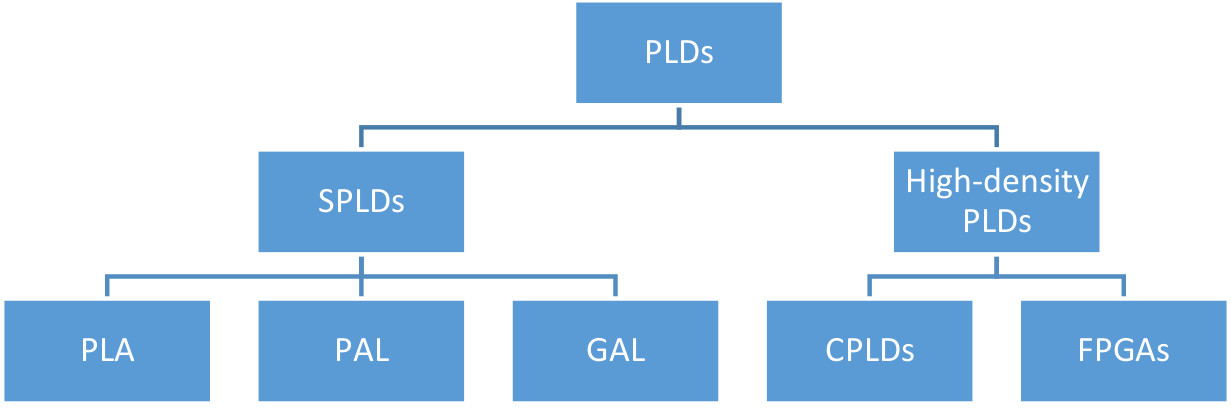
\includegraphics[width=0.8\textwidth]{/home/serga/Desktop/ECE230H/resources/pld_tree.png}
            
            \vspace{0.5cm}

            \textbf{Figure 1: Programmable Logic Device (PLD) Tree Diagram} \autocite{cornell}
            \label{pld_tree_diagram}
        
        \end{center}

        Before understanding what specific programmable devices are and how they 
        function, work needs to be done to understand the basis of all programmable 
        circuits: Programmable Logic Devices, or PLDs. 

        There is a clear structure to the classification of the different types of 
        PLDs. In short, there are two different types of PLDs: Simple Programmable 
        Logic Devices (SPLDs) and High-density PLDs. As shown in 
        \hyperref[pld_tree_diagram]{Figure 1}, there are generally three types of 
        SPLDs, and there are generally two types of High-density PLDs. However, 
        the main difference between the two subcategories, SPLDs and High-density 
        PLDs would be the complexity of the functions they are tasked with. Depending 
        on the design goals of the designer, the scalability of the platform 
        relates to the complexity. In other words, as complexity increases in a 
        highly scalable system, the less likely any undesirable outcomes will 
        hinder design progress, such as added delays and undefined behavior. 
        Inversely, as complexity increases in a not-so-scalable system, the more 
        likely those undesirable outcomes will occur. Overall, the high-density
        PLDs such as CPLDs and FPGAs bring greater scalability compared to their
        SPLD counterparts.

    % This is a citation \citep{social-media-family}.
    % This is a citation \autocite[123]{social-media-family}.
    \section{Device Overview}
        
        \subsection{Programmable Logic Array (PLA)}

        Think of a cooking show. The area where all of the chefs/contestants cook is
        an array of cooking stations. However, the host, or the master chef, of the 
        cooking show decides to equip each cooking station with different utensils 
        and ingredients. The master chef (programmer) can rearrange and configure 
        each of the stations to force the contestants to create a wide variety of 
        dishes based on specific recipes (functions). 

        A PLA typically consists of many programmable AND and OR gates in addition
        to output flip-flops. The programmability of the PLA lies in the user's
        ability to configure the connections between the gates to end up creating
        custom logic functions. The way that PLAs get programmed is through a "PLA
        device programmer" such as PROMs and EPROM-based logic devices 
        \autocite{cornell}. 

        \subsubsection{Programmable Logic Array (PLA) vs. Programmable Array Logic (PAL)}

        Another logic computing device that neighbors the PLA in nomenclature
        is the Programmable Array Logic (PAL) architecture. Although they sound 
        similar, they are not the same. The PAL logic has less complexity compared 
        to the PLA, as the PALs OR matrix is fixed. PLAs offer more complexity by 
        having both a programmable AND and OR matrix. Both architectures will be 
        discussed further, below.
        
        \begin{center}
            \vspace{1cm}

            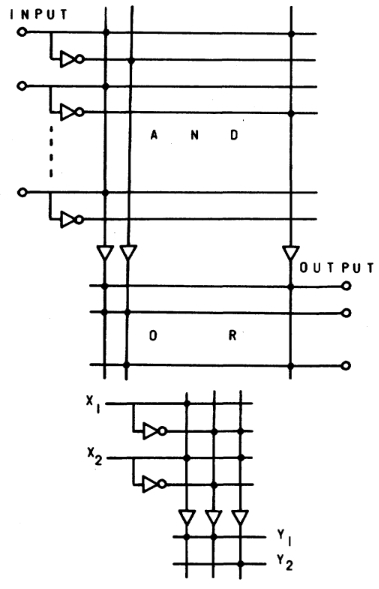
\includegraphics[width=0.4\textwidth]{/home/serga/Desktop/ECE230H/resources/pla_matrix.png}
            
            \vspace{0.5cm}

            \textbf{Figure 2: Programmable Logic Array (PLA) Architecture} \autocite[609]{1675428}
            \label{pla_matrix}
        
        \end{center}

        In general, PLAs can recognize arbitrary logical functions. In 
        \hyperref[pla_matrix]{Figure 2}, there are two parts worth noting: the AND
        matrix and the OR matrix. In the AND matrix, input signals and their 
        inverted counterparts are selectively connected to product term lines in a 
        way such that only specific combinations of input variables produce a 
        combinational output \autocite[609]{1675428}. After, those lines are then
        brought to the second part, the OR matrix. There, other combinational 
        signals transfer the signals to the output lines.

        The inputs to the AND gates are the input variables and their complements 
        (inverted inputs). Within the AND matrix, there are multiple AND gates 
        arranged in a row structure. Each row within the AND matrix corresponds to 
        a different minterm, which is the specific combinational output. This 
        output can be inverted. 

        The output of each AND gate from each row in the AND matrix is connected
        to one input of an OR gate in the OR matrix. The OR matrix receives the
        outputs from the AND matrix and combines them to generate the final output.
        Organizing the structure in this way, the output can be seen in the Sum Of 
        Products (SOP) form.

        Being a \textit{Programmable} Logic Array, it involves some user input to
        enable its potential. Specifically, each of the connections within the 
        AND matrix is programmable. The user can configure which inputs are used 
        in each AND gate. This is done via fuses or antifuses. A fuse in a PLA is
        a low resistive element that could be blown (programmed) to result in an 
        open circuit or high impedance. Inversely, an anti-fuse is a high resistive
        element (initially with high impedance) that can be programmed to result 
        in low impedance \autocite{cornell}. 

    % \paragraph{hello world v2}
        \subsection{Fully Programmable Gate Array (FPGA)}

        After recognizing the nature of PLAs, FPGAs will reach a whole new level of
        complexity. Picture it as a platform where digital architects (programmers) 
        can craft their unique city of logic, complete with streets (interconnects), 
        buildings (logic elements), and adaptable infrastructure - it's a large 
        scale network.

        \begin{center}
            \vspace{0.15cm}

            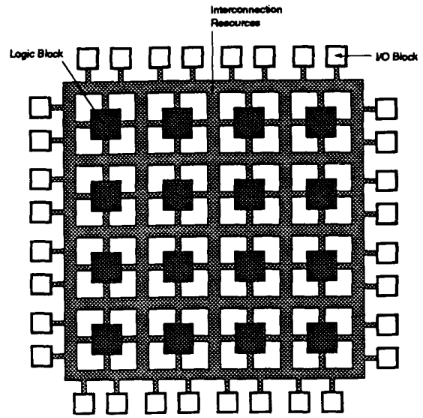
\includegraphics[width=0.4\textwidth]{/home/serga/Desktop/ECE230H/resources/fpga_city.png}
            
            \vspace{0.5cm}

            \textbf{Figure 3: Fully Programmable Gate Array (FPGA) Architecture} \autocite[1013]{231340}
            \label{fpga_city}
        
        \end{center}

        \begin{center}
            \vspace{0.5cm}

            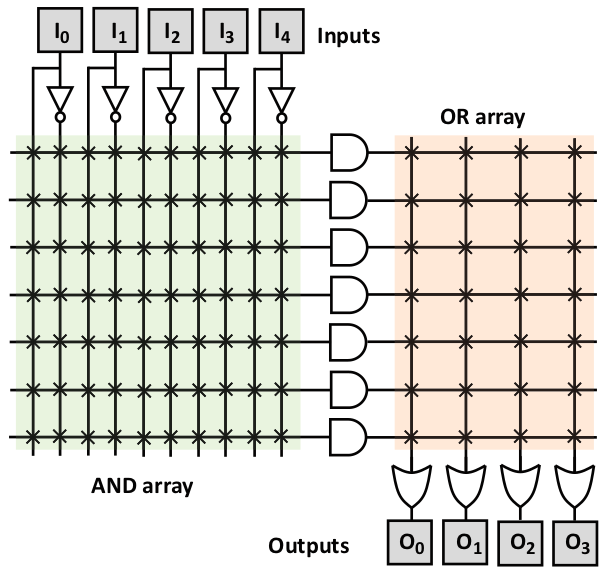
\includegraphics[width=0.4\textwidth]{/home/serga/Desktop/ECE230H/resources/pal_matrix.png}
            
            \vspace{0.5cm}

            \textbf{Figure 4: Programmable Array Logic (PAL) Architecture} \autocite[8]{Boutros2022}
            \label{pal_matrix}
        
        \end{center}

        Compared to the aforementioned Programmable Logic Array, the FPGA is more
        complex. The FPGA is more than the apparent AND-OR matrix structure seen in
        \hyperref[pla_matrix]{Figure 2}. Each of the full-black squares in 
        \hyperref[fpga_city]{Figure 3} represent "logic blocks," which can vary 
        from being as simple as a transistor or as complex as a microprocessor 
        \autocite[1013]{231340}. Essentially, the logic blocks serve as a modular 
        unit within the FPGA, as it is where the digital logic functions are 
        implemented. The channels going in between each of the logic blocks are
        the programmable interconnects. Programmable interconnects are crucial for
        the functionality of the FPGA since they are responsible for connecting the
        matrix together. That way, different logic elements can be used when 
        constructing an implementable design. Another component of the FPGA would
        be the IO blocks. The IO blocks can be reconfigured to adapt to many
        different platforms depending on the design requirements.

        To expand on the topic of logic blocks within an FPGA, they represent the
        core of FPGAs and demonstrate high flexibility and adaptability, not to 
        mention, modularity. Each logic block can be configured to implement 
        arbitrary logic functions. The earliest reconfiguring computing devices were
        Programmable Array Logic (PAL) architectures, as seen in 
        \hyperref[pal_matrix]{Figure 4}, not to be confused with the 
        Programmable Logic Array (PLA) architecture \autocite[8]{Boutros2022}. The
        PAL architecture had its shortcomings. In fact, its main drawback was the 
        scalability factor. As the complexity of the device logic increased, the 
        wires connecting the AND and OR gates together also increased, resulting in 
        a longer execution delay. As a result, the number of required programmable 
        switches grew quadratically \autocite[8]{Boutros2022}. In short, the design 
        of an FPGA takes the PAL architecture and scales it up to many 
        implementations on the same die. As a result, there are many more 
        possibilities for the configurations of the logic elements. For example, 
        besides the basic logic elements (AND/OR), LUT (Look Up Table) and 
        flip-flop-based architectures are also popular.

        With different CLBs (Configurable Logic Blocks) on the same die, the 
        programmable interconnects can convey information from different
        locations. This turns out to be very powerful, as the CLBs can reference 
        inputs/outputs from other CLBs to develop more complex combinational logic 
        with very little latency/delay. 

        \subsection{Programmable Logic Controller (PLC)}

        A Programmable Logic Controller (PLC) is like a conductor in an orchestra.
        It oversees the intricate performance of an industrial symphony, orchestrating
        a harmonious interplay among machines and processes. Similar to a conductor 
        interpreting a musical score, the PLC interprets a programmed logic,
        transforming inputs from sensors into precise outputs that dictate the rhythm
        and flow of production.

        A PLC is a digital electrical system used in manufacturing that 
        utilizes programmable memory to store practice-oriented control programs. 
        Because of this, a PLC is suitable for combinational control, sequence 
        control, time, count, and arithmetic functions \autocite[1]{Frey2014}. 
        Because of its ability to process digital or analog inputs/outputs, it 
        is used for controlling various machines and processes. 

        \begin{center}
            \vspace{0.5cm}

            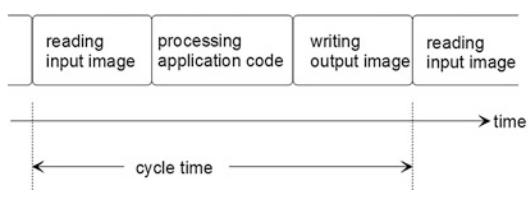
\includegraphics[width=0.55\textwidth]{/home/serga/Desktop/ECE230H/resources/plc_seq.png}
            
            \vspace{0.5cm}

            \textbf{Figure 5: Programmable Logic Controller (PLC) Execution Model} \autocite[2]{Frey2014}
            \label{plc_seq}
        
        \end{center}

        \begin{center}
            \vspace{0.5cm}

            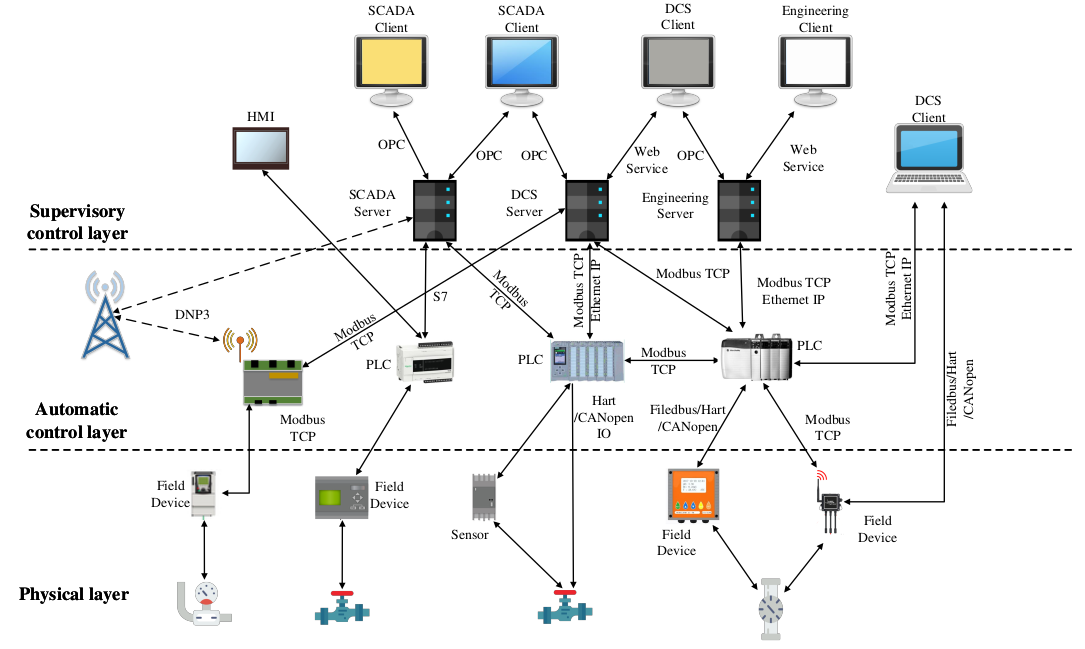
\includegraphics[width=0.95\textwidth]{/home/serga/Desktop/ECE230H/resources/scada_inf.png}
            
            \vspace{0.5cm}

            \textbf{Figure 6: Supervisory Control and Data Acquisition (SCADA) Architecture} \autocite[4]{pr11030918}
            \label{scada_inf}
        
        \end{center}

        Compared to the previously mentioned programmable computing devices, 
        PLAs and FPGAs, PLCs offer more of an industrial application. Where timing 
        is critical and more error prevention/checks are required, PLCs are 
        often apparent. 
        
        When it comes to PLC-based control systems, a Supervisory 
        Control and Data Acquisition (SCADA) system is the most typical 
        \autocite[3]{pr11030918}. SCADA refers to a system of hardware and 
        software components that work together to monitor, control, and manage
        industrial processes, facilities, and infrastructure in real-time. SCADA 
        systems constantly monitor threats and failures in the whole system. This 
        is crucial since any potential attack, failure, or threat could have a 
        significant impact on any of the interdependent critical systems 
        \autocite[121]{Alcaraz2012}. 
        
        The interaction between a PLC and Field Device,
        such as an FPGA is demonstrated in \hyperref[scada_inf]{Figure 6}. The 
        Field Device receives input data and sends it to a PLC via a communication
        protocol such as CAN. From there, the PLC communicates with database 
        servers to store time series data. Any client device can then monitor the
        data coming from the database. Conversely, the PLCs themselves can 
        communicate with the field device to trigger an actuator. Alternatively,
        client devices can interact with a web service to accomplish the same task.
        This example of the interaction between the PLC and the system makes
        them useful for device monitoring and actuation as they can both log 
        critical data and actuate other devices.
        
        \hyperref[plc_seq]{Figure 5} shows the typical deterministic execution
        and software model associated with PLCs. Throughout each program cycle, 
        the PLC reads an image and processes it through various functions to 
        produce an output. The output is often an instruction for actuation.

        Even though the time needed for data acquisition and output writing is 
        constant throughout each program cycle, the time for program execution may
        vary due to the conditional execution of some program parts 
        \autocite[2]{Frey2014}. The benefits of this show through some other 
        capabilities of a PLC: open-loop and closed-loop control. Both these 
        control methods rely either on a constant flow of data or feedback based 
        on a discrete-time control algorithm. Overall, PLCs are a major component
        of control systems that interact with the real world.

        It should come as no surprise that the PLC program (software) directs the 
        PLC (hardware). However, there are different graphical ways to do this. 
        Namely, the Ladder Diagram (LD), and the Function Block Diagram (FBD).
        Initially, the first implementations of LD on the first PLC were intended
        to allow easy access for the people doing hardwired relay logic 
        \autocite[3]{Frey2014}. Now, FBD programs such as MATLAB Simulink are widely 
        available.

        
    \section{Conclusion}
    
    Engineers from all over the world have made it easier for regular consumers
    and other engineers alike to get their hands on digital logic control. 
    Fundamentally, it all started just from simple logic gates. Now, those simple 
    logic gates are incredibly minute building blocks for the bigger picture. Today's
    controllers have way more capabilities than they did decades ago. All of which
    have increased scalability and modularity to tackle future problems.
    
    \subsection{Personal Connection}

    Currently, I am developing a Vehicle Control Unit (VCU) on an 
    embedded controller (PLC) for a Battery Electric Vehicle (BEV) race car using MATLAB 
    Simulink/C for low-level resource management and vehicle state control. 
    I am dealing with discrete-time and varying execution timing with my control 
    algorithms, using both open-loop and closed-loop algorithms. All of course 
    relying on rigid data acquisition to control systems 
    in a High Voltage (HV), high-performance environment. With that 
    background, I can draw a connection to the application of the theory behind PLCs 
    with SCADA methods for actuation, safety, and system security. 
    
    % \addcontentsline{toc}{section}{Works Cited}
    % \printbibliography
    \newpage
    \phantomsection % Create a phantom section to get the correct page number in the ToC
    \addcontentsline{toc}{section}{Works Cited}
    \printbibliography[title=Works Cited]

    % \bibliographystyle{plainnat}
    % \bibliography{sources}

    \end{document}